%%% -*-LaTeX-*-

\chapter{Implementation Details}

This chapter examines the implementation and encoding decisions.

\section{Language Implementation: Decisions and Alternatives}

SweetPea is an embedded domain specific language, meaning that instead of providing its own syntax and the compiler infrastructure to match, it is instead implemented as a library in an embedding language. Here we look at the choice of embedding language, as well as some choices about boolean encodings.

\subsection{Embedding Language}

The current implementation of SweetPea is embedded in Python; the syntax presented in the example code snippets in chapter 4 are valid python program snippets. The subsystem for encoding the counting constraints is currently implemented in Haskell; an earlier implementation of the user-facing SweetPea syntax was also implemented in Haskell. We chose Haskell as an implementation language because its strong static types and functional purity lent it to verifying the correctness of the system. However, many scientists are familiar with Python, and not with Haskell syntax, so we decided to port the user-facing interface to Python to make it easier for them to use and interface with their existing workflows.

\subsection{Why SAT sampling?}

Why does SweetPea need to use a SAT-sampler? Using a SAT-sampler is like bringing a nuke to a knife fight; if a more straight-forward solution was tractable, it would be much simpler, faster, and more maintainable to use a simple solution.

Recall that the goal is to find an ordering of trials which satisfies the constraints, and to return that valid ordering with uniform probability relative to all the other valid orderings. This means that our search space is the space of all possible orderings of the given set of trials (which may realistically consist of $\sim$120 trials, corresponding to $120!$ orderings), and elements of this search space are specific orderings.

The first straight-forward solution is to try a random element in the search space, and see if that ordering satisfies the constraints. For realistic experiments, we found this approach to be intractable-- the set of solutions is sparse in the search space.

The other simpler solution is to generate all of the valid elements, and then choose uniformly among them. In practice, we also found this approach to be intractable. While the space of solutions was sparse in the search space, it was also far too large to exhaustively generate.

The simplest possible solution, and the one used in practice today by psychologists, is to generate the experimental sequence one trial at a time, backtracking when an assignment is made which violates the constraints. Unfortunately this approach does not produce uniformly probable solutions. Similarly, sampling methods like MCMC would also be able to tractably find solutions, but wouldn't provide any guarantee about their distribution.

For the experimental designs we want to support, we found that the methods mentioned above were either intractable or favored certain satisfying sequences over others. Solving the search problem SweetPea addresses is \#P hard \cite{valiant1979complexity}, and our problem size is too large to use brute force despite the exponentially large space.

SweetPea uses the SAT-sampler Unigen because Unigen implements an approximate sampling method with statistical guarantees. Approximate sampling is a compromise: it allows us to gain traction on the otherwise untractably large space, while nonetheless maintaining strong statistically rigorous guarantees of the distribution of solutions. We use Unigen because implementing the underlying sampling method to work well in practice is complicated and an art; it seemed wiser to rely on an existing implementation rather than re-engineer it. This decision, however, to outsource searching the space to Unigen, came at the cost of encoding the domain specific constraints as a boolean formula. The decision to have SweetPea translate from the high-level domain specific semantics to SAT, as opposed to any other possible search space encoding, is an engineering decision; it comes directly from deciding it was better to rely on Unigen rather than reimplement parts of its strategy. It is conceivable that in the future, SweetPea would be able to compile to other backend representation, amenable to other search strategies.


\subsection{Internal Representations}

As mentioned in the previous chapter, we encode levels by allocating one boolean variable per level to indicate the whether that level is in a selected or unselected state. This isn't the only possible encoding; for instance, an encoding which is more compact in the number of variables would represent the index of the selected level in binary. This is a trade-off between variables and clauses, and without any aprior knowledge about the SAT solver's search strategy we chose the encoding which made it easiest to write the constraints which rely on those variables.


\section{Encoding Counting Constraints with Popcount}
%\cite{tseitin1983complexity}

A fully crossed design specifies that each possible combination of levels occurs once in the design. A realistic experiment may have 7 factors, with 2 levels each, for a total of $2^7$ = 128 trials. Each of the levels will appear in half the trials, which means we need to encode constraints of the form "exactly 64 of these 128 variables must be true". The naive encoding ("these 64, or those 64, or those 64, etc") will have 64 choose 128 clauses, which is $10^{37}$ clauses-- far more than any SAT solver can possibly handle. Therefore, we need to encode these kinds of counting constraints in an encoding which is linear in the number of clauses and variables.

To achieve this linear encoding, we emulate the logic in a \emph{popcount} circuit. A popcount circuit is a piece of hardware built out of logic gates which, given a bit string, reports how many bits of the bit string are set. A popcount circuit is implemented as a series of multi-bit wide adders. To explain how we emulate the logic in these circuits we will start with adders and build up to the popcount circuit.

\subsection{Adders}

First let us consider a half-adder. A half-adder is a circuit which takes two single bit inputs \texttt{a} and \texttt{b} and sets two single bit outputs \texttt{s} ("sum") and \texttt{c} ("carry") according to what the sum of the values of \texttt{a} and \texttt{b} are. The value of the input bits is 1 if that variable is true, and 0 if that variable is false. The output bits are boolean functions of the input bits: \texttt{s = a xor b ; c = a and b}. See \shortfigref{half_adder} for an illustration.

What does it mean for a boolean variable to "equal" some relationship between other boolean variables? Really what we mean here is that their values vary in lock-step; that the variable being bound is true only when the relation is true, and false identically when the relation is false. This means that we can represent a half-adder with the boolean formula:
\texttt{(s iff (a xor b)) and (c iff (a and b))}.

How does using a SAT solver allow us to emulate this circuit? Recall that the solver's job is to return an assignment to each of our variables \texttt{(a, b, c, s)} such that the entire formula.

Let us look at some examples. Lets imagine adding 1 + 1; this means that the full formula we hand to the solver is:
\texttt{(s iff (a xor b))} and \texttt{(c iff (a and b))} and \texttt{(a)} and \texttt{(b)}. See \shortfigref{one_plus_one_cnf} for the DIMACS cnf representation of these boolean clauses.
For the entire formula to be true, each of the and clauses must be true. This trivially means that the assignment for \texttt{a} is true, and \texttt{b} is true. Looking at the more interesting clauses, we know \texttt{s} is true \texttt{iff (a xor b)}. \texttt{a xor b} is false when both \texttt{a} and \texttt{b} are true, so \texttt{s} must be false for that clause to be true. We also know that \texttt{c} is true \texttt{iff (a and b)}, so \texttt{c} must also be true.

This means that for this input, the solver would give us the satisfying assignment:
\begin{verbatim}
a is true
b is true
s is false
c is true
\end{verbatim}

See \shortfigref{one_plus_one_sol} for the solution from the SAT solver given the query in \shortfigref{one_plus_one_cnf}.

We can interpret this to mean that the carry bit is 1, and the sum bit is 0: meaning that 1 + 1 = 2. The rest of the constructions in this section follow this intuition: if we build up logical relationships between boolean variables which emulate circuits which perform the computation we wish perform, and constrain some of the input variables, then SAT solver will find what the values of all the other variables must be.

In practice, we want to use a full-adder rather than a half-adder; the difference is that a full-adder also considers a "carry in" bit. This makes it possible to chain full-adder together into multi-bit wide adders.

There are multiple ways to chain together multiple full-adders. SweetPea uses the simplest option, which is ripple-carry adders. N-bit wide ripple-carry adders chain together n full-adders in the natural way: the sum bits of each successive adder form the sum bits of the solution, while the carry bits chain from one adder to the next.

Alternative ways to build multi-bit adders include carry-lookahead adders and carry-save adders; these circuits were designed as physical circuits which can compute the result of the addition in fewer cycles. In some sense, we are also concerned with how long it takes to compute the result: we would like to use the encodings which are most helpful for the solver. There isn't any reason to believe that using a more complicated multi-bit adder design would result in a more favorable encoding; therefore we decided to use the multi-adder design which is simplest to implement, maintain and debug.

\subsection{Popcount Circuit}

The popcount circuit counts the number of bits which are set in a bitstring by a divide-and-conquer-like technique. We will discuss the process below; refer to \shortfigref{popcount} for a diagram.

Let us work through an example: let us count the number of set bits in a bitstring with 9 bits. The first thing we do is zero-pad the bitstring until the next power of two. This is an encoding choice which allocates extra variables to avoid having to handle edge-cases in our logic by allowing us to always be able to divide-and-conquer neatly.

Next, we will pair up bits in the bitstring, and add those using 8 1-bit adders. These two-bit adders will produce 2-bit solutions. Each of these 8 solutions represents how many bits were set in each of their two bit inputs. We repeat this process until we are left with a single 5-bit solution.

Explicitly, this means that we will pair up each of the two-bit solutions, and add them with 4 2-bit wide adders. These will produce 3 bit solutions. We will then pair up these three-bit solutions, and add them with 2 3-bit adders. This will produce only 2 4-bit solutions. Finally, we can take these 2 4-bit answers and add them together with a 4-bit adder to produce a final 5-bit solution.

This final solution represents the number of bits set in the original bitstring in 5-bit binary. Recall that our desired interface was to specify constraints of the form "of these n variables, exactly k must be true". We can then specify this constraint by setting the bits of the final popcount solution to be exactly the same as the binary representation of k. For example, let us specify that we want exactly 3 of the 9 bit to be true our 9-bit popcount example. Let us call the bits of the solution \texttt{[A, B, C, D, E]}. A 5-bit binary representation of 3 is [0, 0, 0, 1, 1], so we can enforce the desired constraint by stating \texttt{[-A, -B, -C, D, E]}.

We also want to provide an interface for specifying constraints of the form "of these n variables, at least (or at most) k must be true". To encode these constraints, we follow a similar technique: we compute the bits which represent the result of the popcount, and encode k in binary. Then, to enforce the inequality we perform a trick: we rewrite $ k < n $ as $ k - n < 0$. To enforce this at the bit-level we write (-n) by representing it in twos-complement. We can then add k + (-n) using a ripple-carry adder. Then, to ensure that $k + (-n) < 0$ we will force the result of that summation to be negative by forcing the top sum bit to be zero.



\begin{figure}
    \centerline{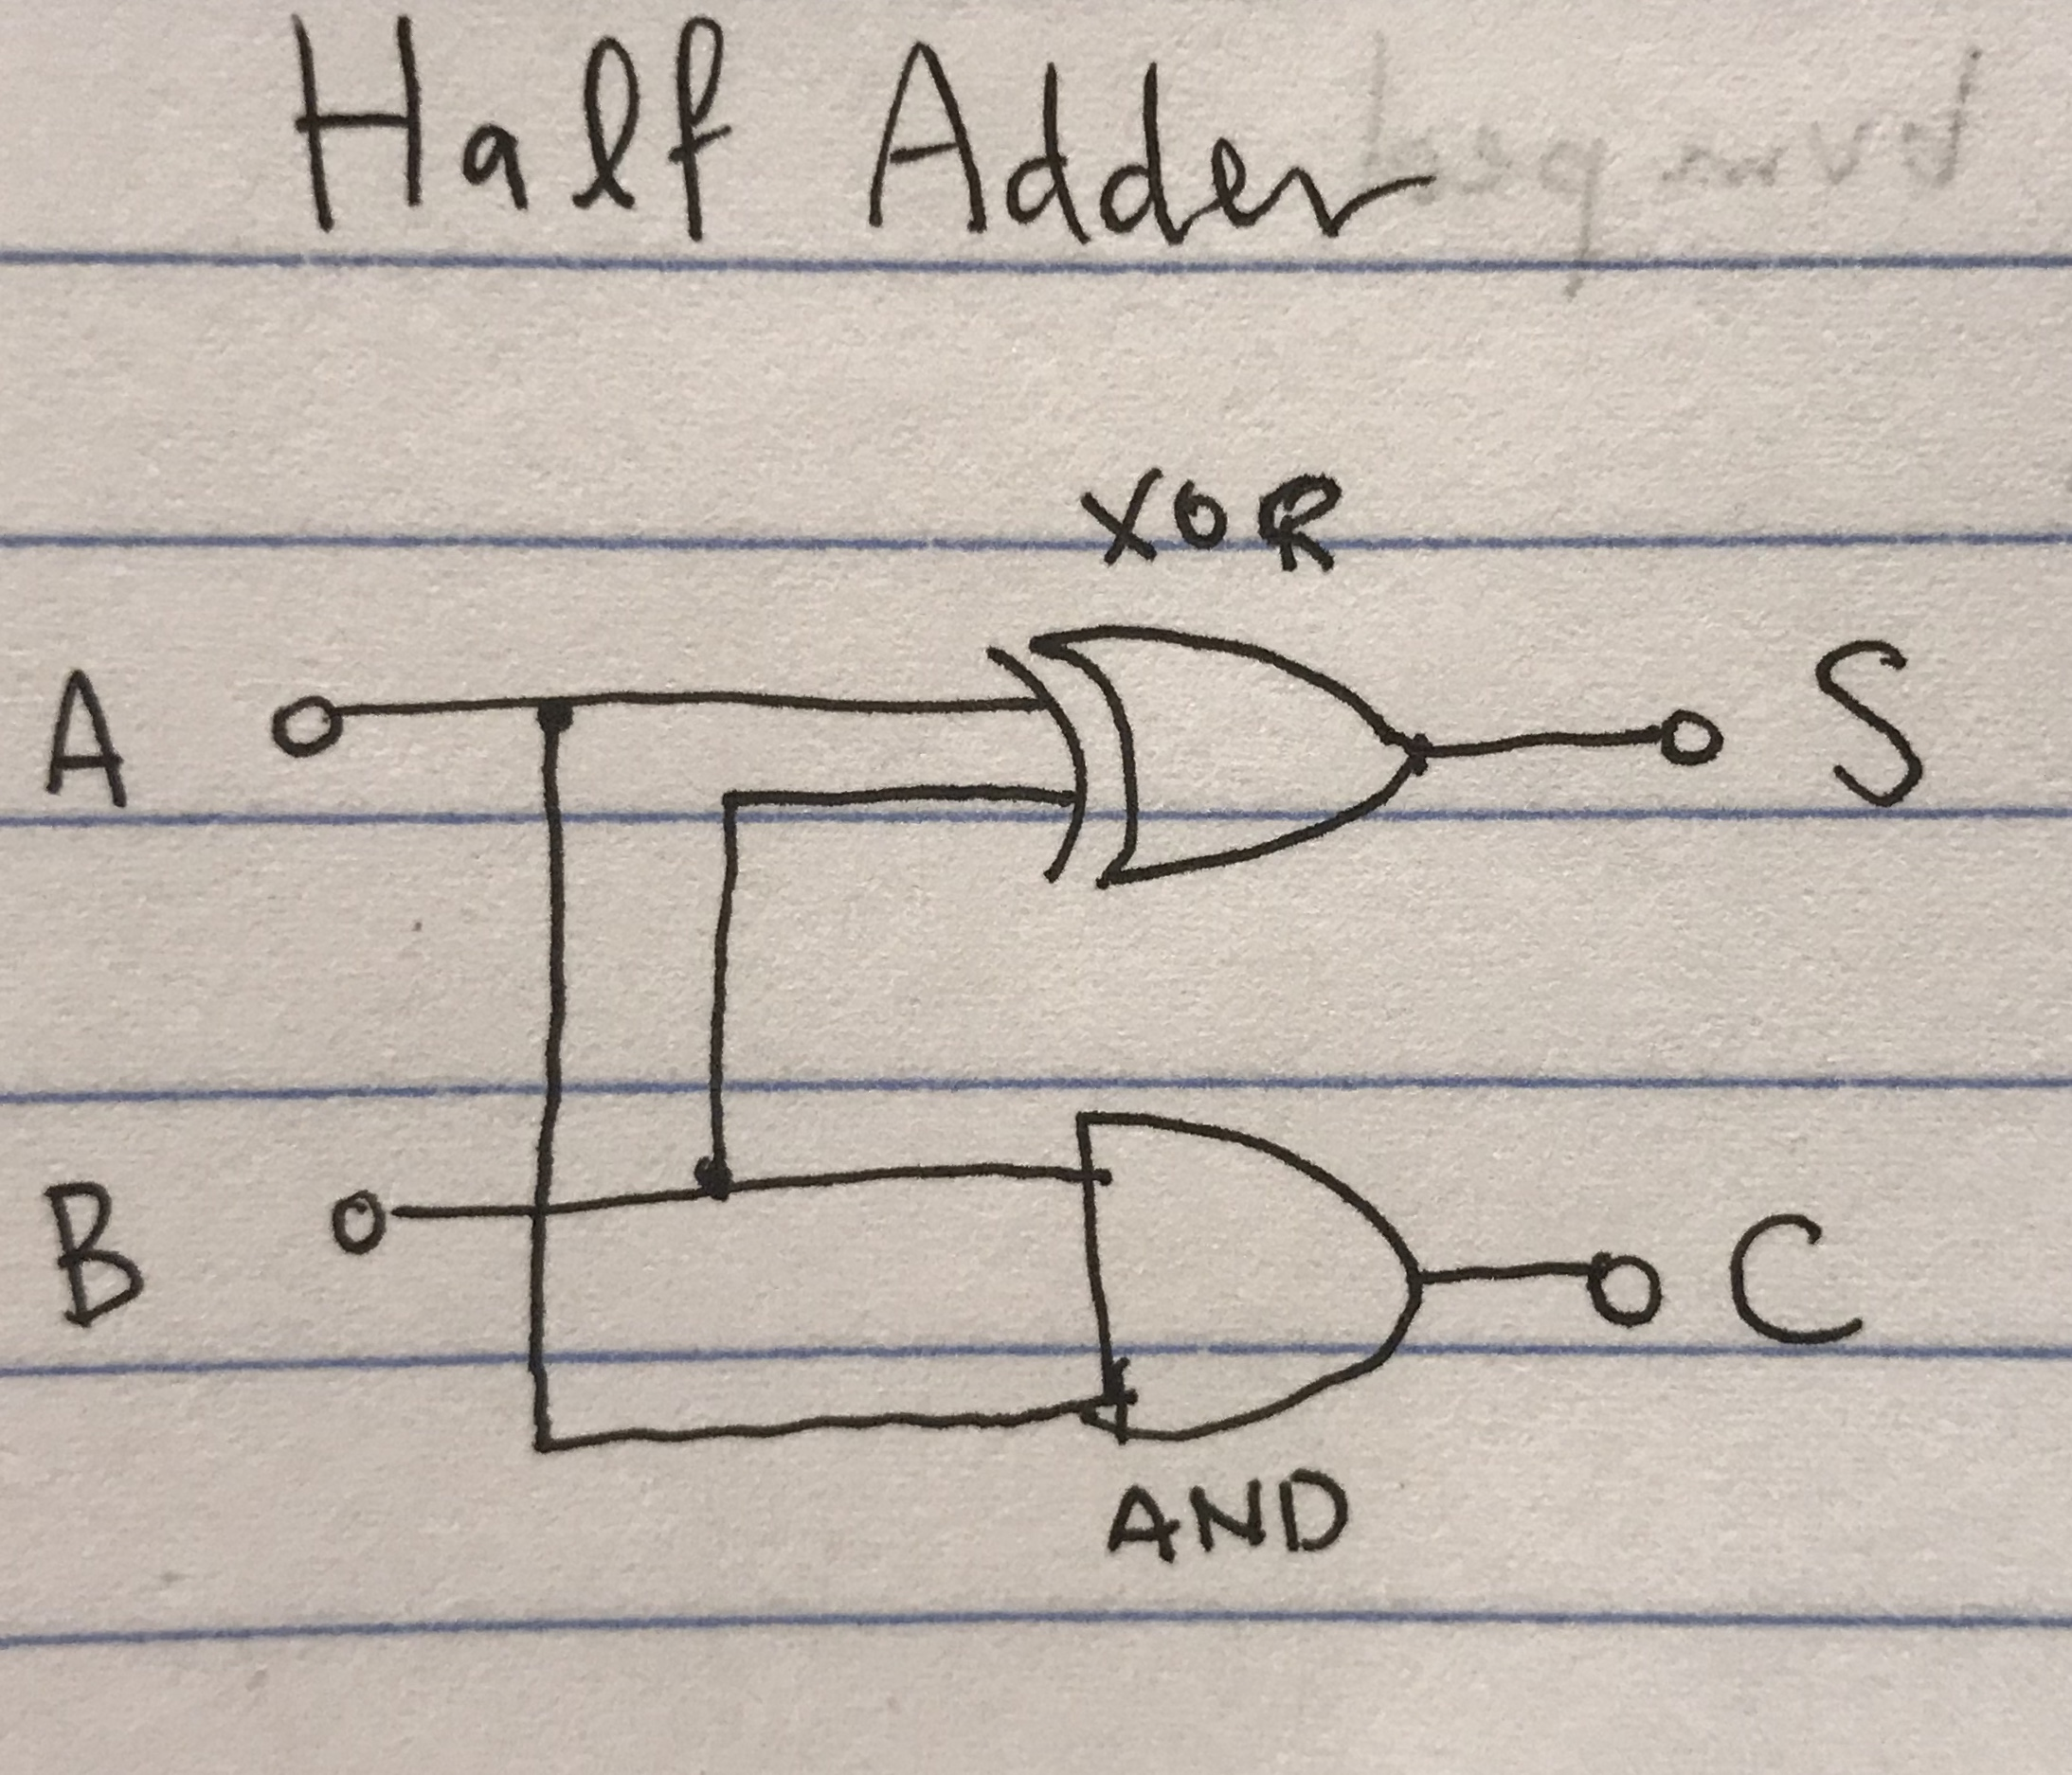
\includegraphics[origin=c,width=6cm]{fig_half_adder}}
    \caption{Half Adder Logic.}%
    \label{fig:half_adder}%
\end{figure}

\begin{figure}
    \centerline{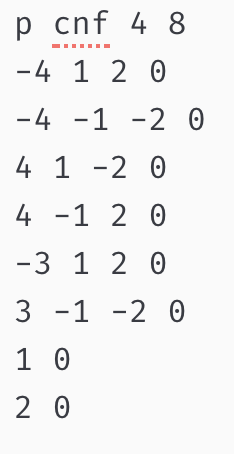
\includegraphics[origin=c,width=2cm]{fig_one_plus_one_cnf}}
    \caption{The DIMACS cnf representation of 1 + 1.}%
    \label{fig:one_plus_one_cnf}%
\end{figure}

\begin{figure}
    \centerline{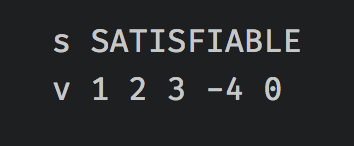
\includegraphics[origin=c,width=2cm]{fig_one_plus_one_sol}}
    \caption{The solution to 1 + 1.}%
    \label{fig:one_plus_one_sol}%
\end{figure}

\begin{figure}
    \centerline{\includegraphics[origin=c,width=15cm]{fig_popcount}}
    \caption{The logic of a popcount circuit.}%
    \label{fig:popcount}%
\end{figure}
